%====================================================================
\chapter{Background}
\label{chap:background}
%====================================================================

% Este capítulo apresenta, de forma abrangente, os conceitos gerais utilizados para compreender e realizar este trabalho.
% A Seção \ref{sec_back:erModel} introduz o modelo entidade-relacionamento, bem como conceitos de modelos lógicos e físicos nas Seções \ref{sec_back:logicalModel} e \ref{sec_back:physicalModel}.
% A Seção \ref{sec_back:mde} apresenta a Model-Driven Engineering e assim suas noções associadas.
% Os conceitos referentes a Domain-Specific Languages são apresentadas na Seção \ref{sec_back:dsl}, seguido de Language Workbenches na Seção \ref{sec_back:LangWorkbench}.
% O Framework Xtext tem uma visão geral exibida na Seção \ref{sec_back:xtext} e, finalmente, as lições do capítulo são discutidas na Seção \ref{sec_back:lessons}.
This chapter presents the general concepts used to understand and implement this work in a comprehensive way.
Section \ref{sec_back:erModel} introduces the entity-relationship model as well as the concepts of logical and physical models in Sections \ref{sec_back:logicalModel} and \ref{sec_back:physicalModel}.
Section \ref{sec_back:mde} introduces Model-Driven Engineering and thus its associated notions.
The concepts referring to Domain-Specific Languages are presented in Section \ref{sec_back:dsl}, followed by Language Workbenches in Section \ref{sec_back:LangWorkbench}.
The Xtext Framework has an overview displayed in Section \ref{sec_back:xtext}, and finally, we discuss the lessons learned in Section \ref{sec_back:lessons}.

%------------------------------------------------------------------------------
\section{Entity-Relationship Model}
\label{sec_back:erModel}
%------------------------------------------------------------------------------

% O modelo conceitual de dados é a descrição de um banco de dado de forma independente da implementação utilizada em um SGBD. 
% Este modelo lista quais dados podem ocorrer no banco de dados, mas não registra como estes dados estão armazenados no nível de SGBD. 
% A técnica mais difundida de modelagem conceitual de dados é a \ac{er} de \cite{Chen:1976}. 
% Esta abordagem foi tão bem aceita que passou a ser considerada uma referência definitiva para a modelagem de bancos de dados relacionais. 
% É composta basicamente por um método de diagramação e de conceitos que devem ser respeitados. 
The conceptual data model is the description of a \ac{db} independently of the implementation used in a \ac{dbms}.
This model lists what data can occur in the \ac{db} but does not record how we stored this data at the \ac{dbms} level.
The most widespread technique of conceptual data modeling is the \ac{er} approach of \cite{Chen:1976}.
This approach was so well accepted that it is now considered a definitive reference for modeling relational \acp{db}.
It is primarily composed of a diagramming method and concepts that must be respected.

% Na abordagem \ac{er} o conceito principal é o de \textbf{entidade}, o qual é uma representação de um conjunto de objetos do domínio modelado \cite{Heuser:2009}. 
% As entidades são simbolizadas por retângulos. 
% Contudo, nesta abordagem ainda existem também outros conceitos que são essenciais e devem ser analisados.
% Para melhor compreensão da modelagem conceitual que utiliza esta abordagem, a seguir são apresentados na Figura \ref{fig:ERConstructors} algumas representações gráficas dos construtores previstos no modelo \ac{er}.
% In the \ac{er} approach, the principal concept is the \textbf{entity}, which is a representation of a set of objects from the modeled domain \cite{Heuser:2009}.
% Entities are symbolized by rectangles.
In the \ac{er} approach, the principal concept is the \textbf{entity}, representing a set of objects from the modeled domain \cite{Heuser:2009}. 
Rectangles symbolize the entities in the diagram. 
However, in this approach there are also other concepts that are essential and should be analyzed. 
For a better understanding of the conceptual modeling that uses this approach, Figure \ref{fig:ERConstructors} presents some graphical representations of the constructors foreseen in the \ac{er} model.

\begin{figure} [!htb]
    \centering
    \caption{ER Model Constructors.}
    \label{fig:ERConstructors}
    

\tikzset{every picture/.style={line width=0.75pt}} %set default line width to 0.75pt        

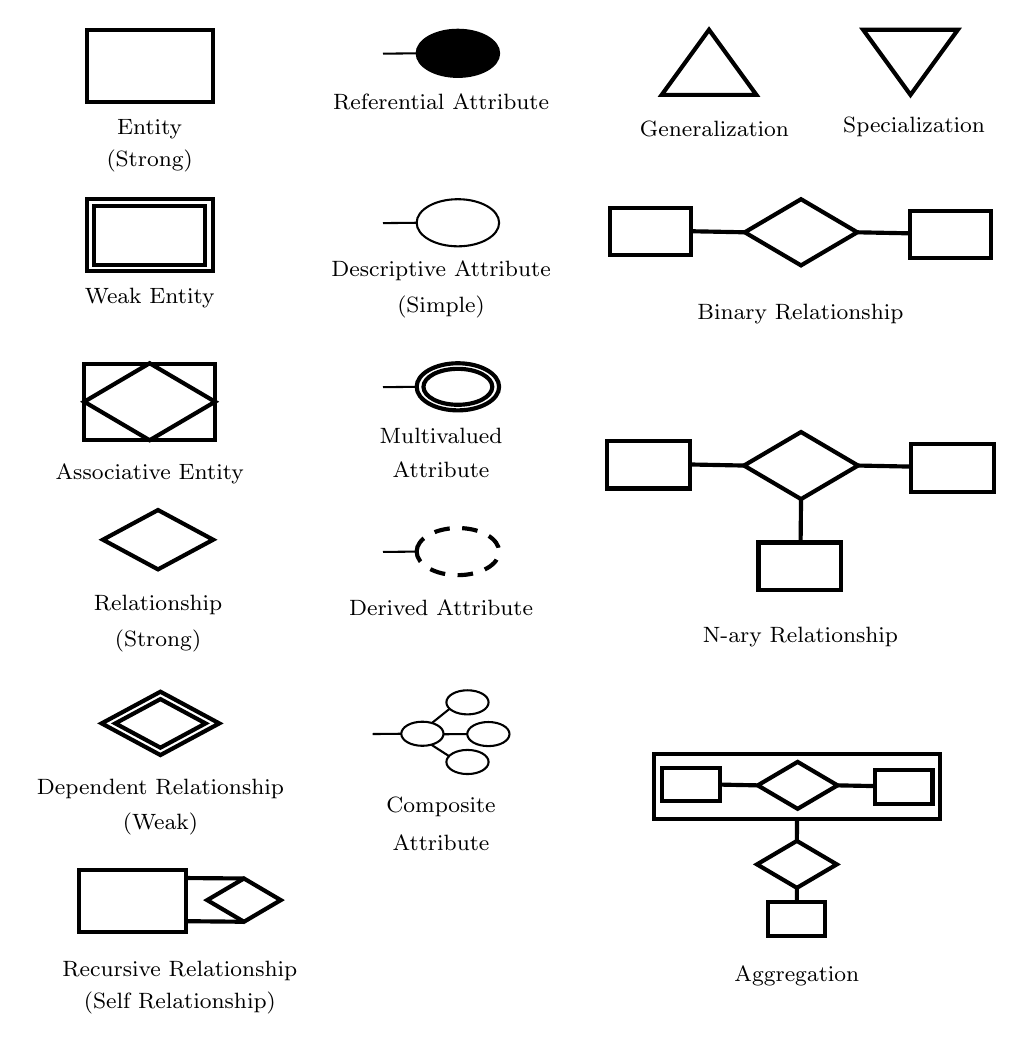
\begin{tikzpicture}[x=0.65pt,y=0.65pt,yscale=-1,xscale=1]
%uncomment if require: \path (0,597); %set diagram left start at 0, and has height of 597

%Shape: Rectangle [id:dp9409938961254447] 
\draw  [line width=1.5]  (29,15) -- (99,15) -- (99,55) -- (29,55) -- cycle ;

%Shape: Rectangle [id:dp25825363492065057] 
\draw  [line width=1.5]  (29,109.2) -- (99,109.2) -- (99,149.2) -- (29,149.2) -- cycle ;
%Shape: Rectangle [id:dp9273607878616594] 
\draw  [line width=1.5]  (33.2,112.8) -- (94.8,112.8) -- (94.8,145.6) -- (33.2,145.6) -- cycle ;

%Shape: Diamond [id:dp07590485693463012] 
\draw  [line width=1.5]  (68.65,282) -- (99.3,298.5) -- (68.65,315) -- (38,298.5) -- cycle ;

%Shape: Diamond [id:dp8393196312653484] 
\draw  [line width=1.5]  (70,383) -- (102.71,400.61) -- (70,418.22) -- (37.29,400.61) -- cycle ;
%Shape: Diamond [id:dp11016744869268091] 
\draw  [line width=1.5]  (70,387.11) -- (95.08,400.61) -- (70,414.11) -- (44.92,400.61) -- cycle ;

%Shape: Ellipse [id:dp8577075014649969] 
\draw   (212.43,122.3) .. controls (212.43,115.07) and (222.69,109.2) .. (235.35,109.2) .. controls (248.01,109.2) and (258.28,115.07) .. (258.28,122.3) .. controls (258.28,129.53) and (248.01,135.4) .. (235.35,135.4) .. controls (222.69,135.4) and (212.43,129.53) .. (212.43,122.3) -- cycle ;
%Straight Lines [id:da240419684606217] 
\draw    (193.72,122.5) -- (212.43,122.3) ;


%Shape: Ellipse [id:dp11655523259938039] 
\draw  [fill={rgb, 255:red, 0; green, 0; blue, 0 }  ,fill opacity=1 ] (212.43,28.1) .. controls (212.43,20.87) and (222.69,15) .. (235.35,15) .. controls (248.01,15) and (258.28,20.87) .. (258.28,28.1) .. controls (258.28,35.33) and (248.01,41.2) .. (235.35,41.2) .. controls (222.69,41.2) and (212.43,35.33) .. (212.43,28.1) -- cycle ;
%Straight Lines [id:da7122954732701139] 
\draw    (193.72,28.3) -- (212.43,28.1) ;


%Shape: Ellipse [id:dp23076223718363464] 
\draw  [line width=1.5]  (212.43,213.5) .. controls (212.43,206.27) and (222.69,200.4) .. (235.35,200.4) .. controls (248.01,200.4) and (258.28,206.27) .. (258.28,213.5) .. controls (258.28,220.74) and (248.01,226.6) .. (235.35,226.6) .. controls (222.69,226.6) and (212.43,220.74) .. (212.43,213.5) -- cycle ;
%Straight Lines [id:da42071644925844054] 
\draw    (193.72,213.7) -- (212.43,213.5) ;
%Shape: Ellipse [id:dp409593727665448] 
\draw  [line width=1.5]  (216.22,213.5) .. controls (216.22,207.99) and (224.78,203.51) .. (235.35,203.51) .. controls (245.92,203.51) and (254.48,207.99) .. (254.48,213.5) .. controls (254.48,219.02) and (245.92,223.49) .. (235.35,223.49) .. controls (224.78,223.49) and (216.22,219.02) .. (216.22,213.5) -- cycle ;


%Shape: Ellipse [id:dp12298573968430726] 
\draw   (203.9,406.37) .. controls (203.9,402.67) and (209.15,399.67) .. (215.63,399.67) .. controls (222.11,399.67) and (227.36,402.67) .. (227.36,406.37) .. controls (227.36,410.07) and (222.11,413.07) .. (215.63,413.07) .. controls (209.15,413.07) and (203.9,410.07) .. (203.9,406.37) -- cycle ;
%Straight Lines [id:da026255036427652145] 
\draw    (187.96,406.53) -- (203.9,406.37) ;
%Shape: Ellipse [id:dp035873659384954015] 
\draw   (228.96,388.9) .. controls (228.96,385.2) and (234.21,382.2) .. (240.69,382.2) .. controls (247.17,382.2) and (252.42,385.2) .. (252.42,388.9) .. controls (252.42,392.61) and (247.17,395.61) .. (240.69,395.61) .. controls (234.21,395.61) and (228.96,392.61) .. (228.96,388.9) -- cycle ;
%Straight Lines [id:da0884897826197295] 
\draw    (220.87,400.43) -- (230.56,392.66) ;
%Shape: Ellipse [id:dp33703819371371857] 
\draw   (240.57,406.54) .. controls (240.57,402.84) and (245.83,399.84) .. (252.31,399.84) .. controls (258.78,399.84) and (264.04,402.84) .. (264.04,406.54) .. controls (264.04,410.24) and (258.78,413.24) .. (252.31,413.24) .. controls (245.83,413.24) and (240.57,410.24) .. (240.57,406.54) -- cycle ;
%Straight Lines [id:da041465674734754376] 
\draw    (227.45,406.65) -- (240.57,406.54) ;
%Shape: Ellipse [id:dp8994114077261279] 
\draw   (228.96,422.06) .. controls (228.96,418.36) and (234.21,415.36) .. (240.69,415.36) .. controls (247.17,415.36) and (252.42,418.36) .. (252.42,422.06) .. controls (252.42,425.77) and (247.17,428.77) .. (240.69,428.77) .. controls (234.21,428.77) and (228.96,425.77) .. (228.96,422.06) -- cycle ;
%Straight Lines [id:da5145813744043246] 
\draw    (220.73,412.57) -- (230.48,418.83) ;


%Shape: Triangle [id:dp717941434970198] 
\draw  [line width=1.5]  (374.97,15) -- (401.3,51.2) -- (348.65,51.2) -- cycle ;

%Shape: Triangle [id:dp8547281306342895] 
\draw  [line width=1.5]  (486.97,51.2) -- (460.65,15) -- (513.3,15) -- cycle ;

%Shape: Ellipse [id:dp057823722753663986] 
\draw  [dash pattern={on 5.63pt off 4.5pt}][line width=1.5]  (212.43,305.1) .. controls (212.43,297.87) and (222.69,292) .. (235.35,292) .. controls (248.01,292) and (258.28,297.87) .. (258.28,305.1) .. controls (258.28,312.33) and (248.01,318.2) .. (235.35,318.2) .. controls (222.69,318.2) and (212.43,312.33) .. (212.43,305.1) -- cycle ;
%Straight Lines [id:da4937273930595423] 
\draw    (193.72,305.3) -- (212.43,305.1) ;


%Shape: Diamond [id:dp8682093873982866] 
\draw  [line width=1.5]  (426.11,109.2) -- (457.39,127.6) -- (426.11,146) -- (394.83,127.6) -- cycle ;
%Shape: Rectangle [id:dp16263593596228687] 
\draw  [line width=1.5]  (319.8,113.94) -- (365.03,113.94) -- (365.03,140.15) -- (319.8,140.15) -- cycle ;
%Shape: Rectangle [id:dp9045715408610813] 
\draw  [line width=1.5]  (486.57,115.67) -- (531.8,115.67) -- (531.8,141.89) -- (486.57,141.89) -- cycle ;
%Straight Lines [id:da894737740624673] 
\draw [line width=1.5]    (366.09,127.03) -- (394.83,127.6) ;
%Straight Lines [id:da45477038200691244] 
\draw [line width=1.5]    (457.39,127.6) -- (486.13,128.17) ;


%Shape: Diamond [id:dp8788662265812572] 
\draw  [line width=1.5]  (426.12,238.62) -- (457.82,257.27) -- (426.12,275.92) -- (394.41,257.27) -- cycle ;
%Shape: Rectangle [id:dp7607057696775741] 
\draw  [line width=1.5]  (318.35,243.42) -- (364.2,243.42) -- (364.2,270) -- (318.35,270) -- cycle ;
%Shape: Rectangle [id:dp20655084709944105] 
\draw  [line width=1.5]  (487.4,245.18) -- (533.25,245.18) -- (533.25,271.76) -- (487.4,271.76) -- cycle ;
%Straight Lines [id:da33926375234409023] 
\draw [line width=1.5]    (365.28,256.69) -- (394.41,257.27) ;
%Straight Lines [id:da8300796405989177] 
\draw [line width=1.5]    (457.82,257.27) -- (486.95,257.85) ;
%Shape: Rectangle [id:dp11640389244166749] 
\draw  [line width=1.5]  (402.47,300.05) -- (448.32,300.05) -- (448.32,326.63) -- (402.47,326.63) -- cycle ;
%Straight Lines [id:da04160890165480735] 
\draw [line width=1.5]    (425.88,299.64) -- (426.12,275.92) ;


%Shape: Diamond [id:dp09298931741553762] 
\draw  [line width=1.5]  (116.43,486.83) -- (136.89,498.86) -- (116.43,510.89) -- (95.98,498.86) -- cycle ;
%Shape: Rectangle [id:dp7562868332770196] 
\draw  [line width=1.5]  (24.66,482.2) -- (84.33,482.2) -- (84.33,516.79) -- (24.66,516.79) -- cycle ;
%Straight Lines [id:da5257649797909345] 
\draw [line width=1.5]    (84.98,510.57) -- (116.43,510.89) ;

%Straight Lines [id:da741474729938117] 
\draw [line width=1.5]    (83.76,486.58) -- (116.43,486.83) ;

%Shape: Diamond [id:dp27975998103917443] 
\draw  [line width=1.5]  (424.23,422.01) -- (446.41,435.06) -- (424.23,448.11) -- (402.04,435.06) -- cycle ;
%Shape: Rectangle [id:dp27388026856661996] 
\draw  [line width=1.5]  (348.82,425.37) -- (380.9,425.37) -- (380.9,443.97) -- (348.82,443.97) -- cycle ;
%Shape: Rectangle [id:dp8682931511633045] 
\draw  [line width=1.5]  (467.12,426.6) -- (499.19,426.6) -- (499.19,445.2) -- (467.12,445.2) -- cycle ;
%Straight Lines [id:da8247964733470876] 
\draw [line width=1.5]    (381.66,434.65) -- (402.04,435.06) ;
%Straight Lines [id:da507174915044009] 
\draw [line width=1.5]    (446.41,435.06) -- (466.8,435.46) ;
%Shape: Diamond [id:dp489563487309699] 
\draw  [line width=1.5]  (423.82,465.94) -- (446,478.99) -- (423.82,492.04) -- (401.63,478.99) -- cycle ;
%Straight Lines [id:da8803188939906841] 
\draw [line width=1.5]    (423.85,453.98) -- (423.82,465.94) ;
%Shape: Rectangle [id:dp2462964817052231] 
\draw  [line width=1.5]  (407.53,500.09) -- (439.61,500.09) -- (439.61,518.68) -- (407.53,518.68) -- cycle ;
%Straight Lines [id:da17335151983105646] 
\draw [line width=1.5]    (423.82,492.04) -- (423.83,500.08) ;
%Shape: Rectangle [id:dp019446741600327666] 
\draw  [line width=1.5]  (344.3,417.82) -- (503.3,417.82) -- (503.3,453.62) -- (344.3,453.62) -- cycle ;


%Shape: Rectangle [id:dp7508437049659447] 
\draw  [line width=1.5]  (27.54,200.66) -- (100.46,200.66) -- (100.46,242.94) -- (27.54,242.94) -- cycle ;
%Shape: Diamond [id:dp4714864707556645] 
\draw  [line width=1.5]  (64,200.4) -- (100.38,221.8) -- (64,243.2) -- (27.62,221.8) -- cycle ;



% Text Node
\draw (64,70) node  [font=\footnotesize] [align=left] {Entity};
% Text Node
\draw (64,88) node  [font=\footnotesize] [align=left] {(Strong)};
% Text Node
\draw (64,164.2) node  [font=\footnotesize] [align=left] {Weak Entity};
% Text Node
\draw (226,55.1) node   [align=left] {{\footnotesize Referential Attribute}};
% Text Node
\draw (226,447) node  [font=\footnotesize] [align=left] {Composite};
% Text Node
\draw (226,467) node  [font=\footnotesize] [align=left] {Attribute};
% Text Node
\draw (226,149.3) node   [align=left] {{\footnotesize Descriptive Attribute}};
% Text Node
\draw (226,169.3) node   [align=left] {{\footnotesize (Simple)}};
% Text Node
\draw (68.65,334.8) node  [font=\footnotesize] [align=left] {Relationship};
% Text Node
\draw (68.65,354.8) node  [font=\footnotesize] [align=left] {(Strong)};
% Text Node
\draw (70,436.8) node  [font=\footnotesize] [align=left] {Dependent Relationship};
% Text Node
\draw (70,456.8) node  [font=\footnotesize] [align=left] {(Weak)};
% Text Node
\draw (226,240.5) node   [align=left] {{\footnotesize Multivalued}};
% Text Node
\draw (226,259.5) node   [align=left] {{\footnotesize Attribute}};
% Text Node
\draw (489,69) node  [font=\footnotesize] [align=left] {Specialization};
% Text Node
\draw (226,336.1) node   [align=left] {{\footnotesize Derived Attribute}};
% Text Node
\draw (378,70) node  [font=\footnotesize] [align=left] {Generalization};
% Text Node
\draw (425.8,352.42) node  [font=\footnotesize] [align=left] {N-ary Relationship};
% Text Node
\draw (425.8,173.22) node  [font=\footnotesize] [align=left] {Binary Relationship};
% Text Node
\draw (423.8,541.2) node  [font=\footnotesize] [align=left] {Aggregation};
% Text Node
\draw (80.78,538.2) node  [font=\footnotesize] [align=left] {Recursive Relationship};
% Text Node
\draw (80.78,556.2) node  [font=\footnotesize] [align=left] {(Self Relationship)};
% Text Node
\draw (64,262.2) node   [align=left] {{\footnotesize Associative Entity}};


\end{tikzpicture}

    \fonte{Author.}
\end{figure}

% Uma \textbf{Entidade Forte} e uma entidade que para existir não depende da existência de outra(s) entidades(s). 
% De forma inversa, uma \textbf{Entidade Fraca} é uma entidade que possui sua existência ou identificação dependente de outra(s) entidade(s). 
% A representação de \textbf{Entidade Associativa} serve para dar mais sentido semântico ao modelo, e pode ser usada para simbolizar relações muitos para muitos, contendo referências a colunas de tabelas do mesmo ou de outros \acp{db}.
A \textbf{strong entity} is an entity that does not depend on the existence of other entity(ies) to exist.
Conversely, a \textbf{weak entity} is an entity that has its existence or identification dependent on other entity(ies).
An \textbf{associative entity} serves to give more semantic meaning to the model and to symbolize many-to-many relationships, containing references to columns of tables of the same or other \acp{db}.

% Os \textbf{atributos} podem ser \textbf{referenciais}, ou seja, que identificam a entidade, e \textbf{descritivos} que a descrevem. 
% A maioria dos atributos tendem a ser descritivos e também são chamados de simples ou monovalorados. 
% Contudo, existem outros tipos destes atributos como os \textbf{multivalorados}, que podem assumir diversos valores, os \textbf{derivados}, que são inferidos a partir de outros atributos, e os \textbf{compostos}, que podem ser divididos em várias partes com significados independentes.
The \textbf{attributes} can be \textbf{referential}, that is, they identify the entity, and \textbf{descriptive} that describe it.
Most attributes tend to be descriptive and are also called simple or single-valued.
However, there are other types of these attributes such as \textbf{multi-valued}, which can take different values, \textbf{derived}, which are inferred from other attributes, and \textbf{composite} attributes, which can be divided into several parts with independent meanings.

% No que diz respeito aos \textbf{relacionamentos} possíveis entre entidades pode-se citar os \textbf{binários}, aqueles que envolvem duas (2) entidades, e os \textbf{n-ários} que correspondem a ligação de três (3) ou mais entidades. 
% É comum que as relações compostas especificamente por três entidades sejam chamadas de relações \textbf{ternárias}. 
% Além destes tipos ainda é possível haver relações recursivas de uma entidade com ela mesma, também chamado de \textbf{auto-relacionamento}.
Regarding the possible \textbf{relationships} between entities, we can mention the \textbf{binary} that involve two (2) entities and the \textbf{n-ary} that correspond to the link of three (3) or more entities.
It is common for relations composed of three entities to be called \textbf{ternary} relations.
Besides these types, it is still possible to have recursive relationships of an entity with itself, also called \textbf{self-relationship}.

% A abordagem \ac{er} ainda suporta conceitos de \textbf{generalização/especialização}, que definem um grupo hierárquico de entidades que compartilham atributos em comum, e \textbf{agregação} onde a condição de existência é que o relacionamento principal necessita ser necessariamente de muitos para muitos.
The \ac{er} approach still supports concepts of \textbf{generalization/specialization}, which define a hierarchical group of entities that share common attributes, and \textbf{aggregation} where the existence condition is that the principal relationship needs to be necessarily from many-to-many.

% Os \textbf{relacionamentos} representam a associação entre os objetos e são sinalizados por losangos. 
% A \textbf{cardinalidade} de relacionamentos registra o número de ocorrências com que as entidades podem se associar. 
% Existem duas cardinalidades que devem ser atribuídas: a mínima e a máxima. 
% Os \textbf{atributos} são características representadas por pequenos círculos conectados as entidades. 
The \textbf{relationships} represent the association among objects, and diamonds denote them.
The \textbf{cardinality} of relationships records the number of occurrences that entities can associate with each other.
Two cardinalities must be assigned: the minimum and the maximum. \textbf{Attributes} are features represented by small circles connected to entities.

%------------------------------------------------------------------------------
\section{Logical Model}
\label{sec_back:logicalModel}
%------------------------------------------------------------------------------

% Um modelo lógico de dados é definido como um modelo que possui a representação dos objetos, relacionamentos e características de acordo com regras de implementação. 
% Isso significa que esse modelo tem um nível de abstração do ponto de vista do usuário de um \ac{dbms}. 
% Ainda assim, o modelo lógico é independente do tipo de \ac{dbms} em que é implementado. 
A logical data model defines a model that represents objects, relationships, and characteristics according to implementation rules.
This means that this model has a level of abstraction from the user's point of view of a \ac{dbms}.
Still, the logical model is independent of the type of \ac{dbms} in which that implements it.

% Esse tipo de modelo deve necessariamente respeitar conceitos tais como chaves de acesso, controle de chaves duplicadas, normalização, integridade referencial, controle de redundância de dados, entre outros. 
% Este modelo é intrinsecamente relacionado a fase de projeto \cite{Cougo:2013}. 
% É importante salientar que essa é uma forma direcionada a um aspecto gráfico, porém existem meios alternativos de se representar estruturalmente o mesmo modelo de forma textual \cite{Martelli:2018}. 
This type of model must necessarily respect concepts such as access keys, duplicate keys control, normalization, referential integrity, data redundancy control, among others.
This model is intrinsically related to the design phase \cite{Cougo:2013}.
% It is important to point out that this is a form directed to a graphic aspect, but there are alternative ways to structurally represent the same model in a textual form \cite{Martelli:2018}.
It is worth pointing out that this is a directed way to graphical aspect, but there are alternative ways to represent the same structurally model in a textual form \cite{Martelli:2018}.

%------------------------------------------------------------------------------
\section{Physical Model}
\label{sec_back:physicalModel}
%------------------------------------------------------------------------------

% Um modelo físico de dados caracteriza-se como um modelo em que a representação dos objetos de \ac{db} já estão em um nível físico de implementação das ocorrências, ou instâncias, das entidades de relacionamentos. 
% Cada \ac{dbms} pode definir diferentes modos de implementação física das características e recursos indispensáveis para o armazenamento e manipulação das estruturas de dados \cite{Cougo:2013}.
A physical data model characterizes as a model in which the \ac{db} objects representation are already at a physical level of implementation of the occurrences (or instances) of the entities of relationships.
Each \ac{dbms} can define different modes of physical implementation, involving characteristics and essential resources for the storage and manipulation of data structures. \cite{Cougo:2013}.

% Em geral os modelos físicos apresentam dois aspectos bem representados. 
% Primeiramente, existem as ocorrências ou instâncias, seus relacionamentos e a disposição básica dos elementos. 
% O outro aspecto diz respeito a alocação nos diversos níveis de agrupamentos possíveis, como as tabelas, linhas (registros), colunas (campos) e blocos \cite{West:2011}.
% Em suma, é a materialização dos objetos de \ac{db} em um esquema interno de um dado \ac{dbms} a partir da execução de uma sequência lógica de instruções em \ac{sql}.
In general, physical models have two well-represented aspects.
First, there are the occurrences or instances, their relationships, and the basic arrangement of elements.
The other aspect concerns the allocation in the different levels of possible groupings, such as tables, rows (records), columns (fields), and blocks \cite{West:2011}.
In short, it is the materialization of \ac{db} objects in an internal schema of a given \ac{dbms} from the execution of a logical sequence of instructions in \ac{sql}.

%------------------------------------------------------------------------------
\section{Model-Driven Engineering}
\label{sec_back:mde}
%------------------------------------------------------------------------------

% Conceitualmente um modelo é uma representação, protótipo ou exemplo que se tem por objetivo reproduzir ou imitar alguma forma. 
% A construção de modelos são pontos centrais e importantes em diferentes áreas científicas. 
% Na matemática, física, engenharia e química, por exemplo, o emprego de modelos é tido como vital para a investigação teórica e prática em diferentes campos de estudo \cite{Bailer:2009}.
A model is, conceptually, a representation, prototype or example that has the objective of reproducing or imitating something in some way.
Model building is central and relevant in different scientific areas.
In mathematics, physics, engineering, and chemistry areas, for example, the use of models is considered vital for theoretical and practical research in different fields of study \cite{Bailer:2009}.

% A \ac{mde}, ou \ac{mdse}, é um campo da Engenharia de Software que tem sua origem a partir da criação das primeiras ferramentas CASE surgidas nos anos 1980.
% Enquanto subárea da Engenharia de Software, a \ac{mde} é uma abordagem que preconiza essencialmente que um processo de desenvolvimento tenha modelos como principais saídas (ou também como entradas) de alguma atividade.  
% Esta abordagem tem como objetivo maximizar a produtividade, a compatibilidade entre sistemas (através da reutilização de modelos) e simplificar a complexidade envolvida no processo de projeto de software \cite{Brambilla:2017}. 
% Dessa forma, isto resulta em programas ou atividades de computador executados em hardware ou software que são gerados automaticamente a partir de modelos \cite{Sommerville:2011}. 
\ac{mde}, or \ac{mdse}, is a field of Software Engineering that has its origins since the creation of the first \ac{case} tools that emerged in the 1980s.
As a sub-area of Software Engineering, \ac{mde} is an approach that essentially calls for a development process to have models as the main inputs (or also outputs) of some activity.
This approach aims to maximize productivity, compatibility between systems (through model reuse) and simplify the complexity involved in the software design process  \cite{Brambilla:2017}.
In this way, this results in programs or computer activities executed in hardware or software that are automatically generated from models \cite{Sommerville:2015}.

% Esta área de estudo vem evoluindo consideravelmente desde os anos 1990. 
% Em resumo,  a MDE fez contribuições para potencializar a abstração, visando assim a automação, em quase todas as áreas de desenvolvimento e análise \cite{Bucchiarone:2020}. 
% Essas contribuições podem ser identificadas em diversos domínios onde modelos são indispensáveis para o sucesso e.g. sistemas de software, sistemas de transporte, indústria automotiva, processos de negócio, biotecnologia e genética. 
% Conceitualmente, a \ac{mde} fornece apoio a outros conceitos, como o \ac{mdd} e a \ac{mda}. Na Figura \ref{fig:MDE} a relação entre estes conceitos é ilustrada
This area of study has been evolving considerably since the 1990s.
In short, MDE has made contributions to leverage abstraction, thus aiming at automation, in almost all areas of development and analysis \cite{Bucchiarone:2020}.
These contributions identified in several domains where models are indispensable for success e.g. software systems, transport systems, automotive industry, business processes, biotechnology, and genetics.
Conceptually, \ac{mde} supports other concepts such as \ac{mdd} and \ac{mda}. 
Figure \ref{fig:MDE} illustrates the relationship among these concepts.
% In Figure \ref{fig:MDE} the relationship between these concepts is illustrated.

\begin{figure}[!htb]
    \centering
    \caption{Relationship among MDE, MDD and MDA.}
    

\tikzset{every picture/.style={line width=0.75pt}} %set default line width to 0.75pt        

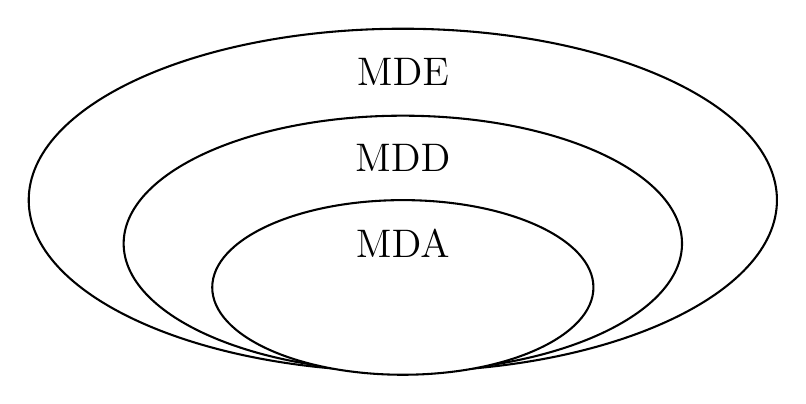
\begin{tikzpicture}[x=0.75pt,y=0.75pt,yscale=-1,xscale=1]
%uncomment if require: \path (0,300); %set diagram left start at 0, and has height of 300

%Shape: Ellipse [id:dp03875628946363818] 
\draw  [fill={rgb, 255:red, 255; green, 255; blue, 255 }  ,fill opacity=1 ] (91,113.58) .. controls (91,67.97) and (171.7,31) .. (271.25,31) .. controls (370.8,31) and (451.5,67.97) .. (451.5,113.58) .. controls (451.5,159.18) and (370.8,196.15) .. (271.25,196.15) .. controls (171.7,196.15) and (91,159.18) .. (91,113.58) -- cycle ;
%Shape: Ellipse [id:dp565416950765411] 
\draw  [fill={rgb, 255:red, 255; green, 255; blue, 255 }  ,fill opacity=1 ] (136.74,134.53) .. controls (136.74,100.49) and (196.96,72.9) .. (271.25,72.9) .. controls (345.54,72.9) and (405.76,100.49) .. (405.76,134.53) .. controls (405.76,168.56) and (345.54,196.15) .. (271.25,196.15) .. controls (196.96,196.15) and (136.74,168.56) .. (136.74,134.53) -- cycle ;
%Shape: Ellipse [id:dp0635650382067301] 
\draw  [fill={rgb, 255:red, 255; green, 255; blue, 255 }  ,fill opacity=1 ] (179.42,155.65) .. controls (179.42,132.41) and (220.53,113.58) .. (271.25,113.58) .. controls (321.97,113.58) and (363.08,132.41) .. (363.08,155.65) .. controls (363.08,178.88) and (321.97,197.72) .. (271.25,197.72) .. controls (220.53,197.72) and (179.42,178.88) .. (179.42,155.65) -- cycle ;

% Text Node
\draw (271.25,52) node  [font=\Large] [align=left] {MDE};
% Text Node
\draw (271.25,93) node  [font=\Large] [align=left] {MDD};
% Text Node
\draw (271.25,134.65) node  [font=\Large] [align=left] {MDA};


\end{tikzpicture}

    \fonte{Adapted from \cite{Ameller:2009}}
    \label{fig:MDE}
\end{figure}

% O \ac{mdd} é um paradigma de desenvolvimento que usa modelos como principais artefatos em um processo de desenvolvimento. 
% No \ac{mdd} geralmente a implementação é gerada de forma automática ou semiautomática a partir dos modelos. 
% Apesar de serem vistas como a mesma coisa, os conceitos estabelecidos na literatura acerca da \ac{mde} e da \ac{mdd} tem origem direta na \ac{mda}, formalmente proposta inicialmente em 2001 pela \ac{omg}\footnote{MDA Guide 2.0: \url{ https://www.omg.org/cgi-bin/doc?ormsc/14-06-01.pdf}}. 
\ac{mdd} is a development paradigm that uses models as principal artifacts in a development process.
In \ac{mdd}, the implementation is usually generated automatically or semi-automatically from the models.
Despite being seen as the same thing, the concepts established in the literature about \ac{mde} and \ac{mdd} have direct origins in \ac{mda}, first formally proposed only in 2001 by \ac{omg}\footnote{MDA Guide 2.0: \url{ https://www.omg.org/cgi-bin/doc?ormsc/14-06-01.pdf}}.

% Segundo \cite{Sommerville:2015} as diferenças são sutis, uma vez que a \ac{mda} concentra-se nos estágios de projeto e implementação do processo de desenvolvimento de software, sendo muito similar ao \ac{mdd}, porém implementando diretrizes específicas da \ac{omg}. 
% Isso faz com que os processos de \ac{mdd} se utilizem de diversas abstrações para esconder, ou até mesmo remover, detalhes que possam eventualmente tornar um modelo mais complexo. 
According to \cite{Sommerville:2015}, the differences are subtle since \ac{mda} focuses on the design and implementation stages of the software development process, being very similar to \ac{mdd}, however implementing \ac{omg}-specific guidelines.
Hence, this causes the \ac{mdd} processes to use various abstractions to hide, or even remove, details that could eventually make a model more complex.

% Dito isto, conclui-se que a \ac{mda} é um subconjunto do \ac{mdd}. 
% Por outro lado, a \ac{mde} pode abordar muitos outros tópicos dos processos de Engenharia de Software, entre eles a engenharia de requisitos baseada em modelos, processos de software para desenvolvimento baseado em modelos, ou ainda, testes baseados em modelos.
% A \ac{mde}, como uma metodologia, auxilia a aplicação das vantagens da modelagem nas atividades de Engenharia de Software. 
% Para \cite{Brambilla:2017} essa abordagem leva em consideração quatro aspectos fundamentais, listados a seguir.

Once that is said, it follows that \ac{mda} is a subset of \ac{mdd}.
On the other hand, \ac{mde} can address many others topics in Software Engineering processes, including model-based requirements engineering, model-based software processes for development, or even model-based testing.
\ac{mde}, as a methodology, helps to apply the advantages of modeling in Software Engineering activities.
For \cite{Brambilla:2017}, this approach takes into consideration four fundamental aspects listed below.

% \begin{enumerate}
%   \item Conceitos: os componentes que constroem a metodologia, abrangendo desde artefatos de linguagem até atores, e assim por diante;
%   \item Notações: A maneira como os conceitos são representados, ou seja, as linguagens usadas na metodologia;
%   \item Processos e Regras: As atividades que levam à elaboração do produto final, as regras para sua administração e controle, e as afirmações sobre as propriedades desejadas (correção, consistência, etc) dos produtos ou do próprio processo;
%   \item Ferramentas: Aplicações que facilitam a execução de atividades ou seu controle, abrangendo o processo de produção e apoiando o desenvolvedor no uso das notações.
% \end{enumerate}

\begin{enumerate}
   \item \textbf{Concepts}: the components that build the methodology, ranging from language artifacts to actors, and so forth;
   \item \textbf{Notations}: The way concepts are represented, \textit{i.e.} the languages used in the methodology;
   \item \textbf{Processes and Rules}: The activities that lead to the elaboration of the final product, the rules for its administration and control, and the statements about the desired properties (correction, consistency, etc) of the products or of the process itself;
   \item \textbf{Tools}: Applications that facilitate the execution of activities or their control, covering the production process, and supporting the developer in the use of notations.
\end{enumerate}

% A motivação por trás da \ac{mde} é a ideia de se aumentar o nível de abstração do processo de desenvolvimento em geral, para então assim capturar sistemas ou processos como uma coleção de modelos reutilizáveis. 
% Logo, ela visa reduzir a dificuldade associada ao desenvolvimento de sistemas de software, em geral mais complexos, por meio do uso de técnicas de modelagem que suportam a separação de interesses e geração automatizada de artefatos de sistemas a partir de modelos \cite{Batory:2015, Kleppe:2003}.
The motivation behind \ac{mde} is increasing the abstraction level of the development process in general and then capturing processes or systems as a collection of reusable models.
Therefore, it aims to reduce the difficulty associated with the development of software systems, which are generally more complex, through the modeling techniques implementation that supports the separation of interests and the automated generation of system artifacts from models \cite{Batory:2015, Kleppe:2003}.
% Therefore, it aims to reduce the difficulty associated with developing software systems, which are generally more complex, through the use of modeling techniques that support the separation of interests and automated generation of system artifacts from models \cite{Batory:2015, Kleppe:2003}.

% De uma forma objetiva, a abordagem \ac{mda} define uma estrutura para se realizar a \ac{mde}, ou também ainda a \ac{mdd}. 
% Essa abordagem define três camadas que devem ser usadas como pilares para todo o processo \cite{Frantz:2012}, listados a seguir.
% A relação conceitual entre esses níveis, com o uso de mecanismos de transformação e regras de transformação, é exemplificado na Figura \ref{fig:MDA}.

Objectively, the \ac{mda} approach defines a structure to perform the \ac{mde}, or also the \ac{mdd}.
% This approach defines three layers that should be used as pillars for the whole process \cite{Frantz:2012} listed below.
This approach defines three layers used as pillars for the whole process \cite{Frantz:2012} listed below.
The conceptual relationship between these levels, using transformation mechanisms and transformation rules, is exemplified in Figure \ref{fig:MDA}.

% \begin{enumerate}
%     \item \acp{CIM}: descrevem objetos de negócio e as atividades independentemente de sistemas de suporte;
%     \item \acp{PIM}: descrevem como os processos de negócio são suportados por sistemas, vistos como caixas-pretas funcionais, ou seja, desconsiderando as restrições associadas às tecnologias candidatas;
%     \item \acp{PSM}: descrevem os componentes do sistema conforme implementados por tecnologias específicas.
% \end{enumerate}
\begin{enumerate}
     \item \textbf{\acp{cim}}: describe business objects and activities independently from support systems;
     \item \textbf{\acp{pim}}: describe how business processes are supported by systems, seen as functional black boxes, \textit{i.e.} disregarding the restrictions associated with candidate technologies;
     \item \textbf{\acp{psm}}: describe system components as implemented by specific technologies.
\end{enumerate}

\begin{figure}[!htb]
    \centering
    \caption{MDA abstraction levels.}
    

\tikzset{every picture/.style={line width=0.75pt}} %set default line width to 0.75pt        

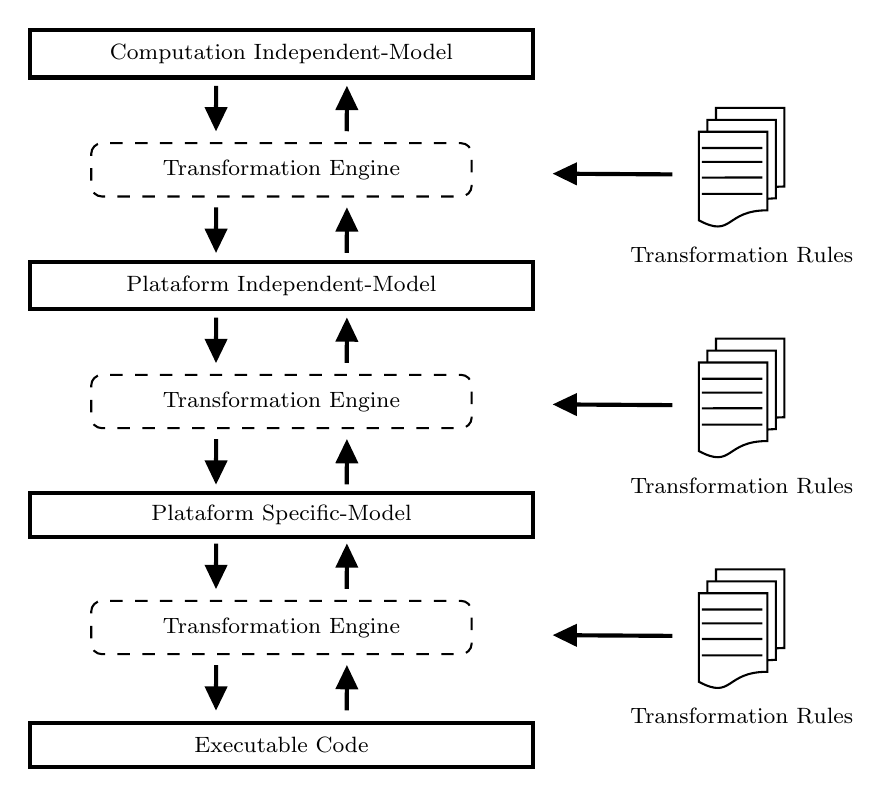
\begin{tikzpicture}[x=0.75pt,y=0.75pt,yscale=-1,xscale=1]
%uncomment if require: \path (0,442); %set diagram left start at 0, and has height of 442

%Shape: Rectangle [id:dp7655816759589134] 
\draw  [fill={rgb, 255:red, 255; green, 255; blue, 255 }  ,fill opacity=1 ][line width=1.5]  (52.59,47.21) -- (295.12,47.21) -- (295.12,70.24) -- (52.59,70.24) -- cycle ;

%Shape: Rectangle [id:dp37583246050722807] 
\draw  [fill={rgb, 255:red, 255; green, 255; blue, 255 }  ,fill opacity=1 ][line width=1.5]  (52.59,159.07) -- (295.12,159.07) -- (295.12,181.86) -- (52.59,181.86) -- cycle ;

%Shape: Rectangle [id:dp8974163182307999] 
\draw  [fill={rgb, 255:red, 255; green, 255; blue, 255 }  ,fill opacity=1 ][line width=1.5]  (52.59,270.24) -- (295.12,270.24) -- (295.12,291.66) -- (52.59,291.66) -- cycle ;

%Shape: Rectangle [id:dp7966059165934565] 
\draw  [fill={rgb, 255:red, 255; green, 255; blue, 255 }  ,fill opacity=1 ][line width=1.5]  (52.59,381.18) -- (295.12,381.18) -- (295.12,402.38) -- (52.59,402.38) -- cycle ;

%Straight Lines [id:da6759491853813937] 
\draw [fill={rgb, 255:red, 255; green, 255; blue, 255 }  ,fill opacity=1 ][line width=1.5]    (142.38,74.28) -- (142.34,92.11) ;
\draw [shift={(142.33,96.11)}, rotate = 270.14] [fill={rgb, 255:red, 0; green, 0; blue, 0 }  ][line width=0.08]  [draw opacity=0] (11.61,-5.58) -- (0,0) -- (11.61,5.58) -- cycle    ;
%Straight Lines [id:da4410578197502153] 
\draw [fill={rgb, 255:red, 255; green, 255; blue, 255 }  ,fill opacity=1 ][line width=1.5]    (205.33,96.11) -- (205.38,78.28) ;
\draw [shift={(205.39,74.28)}, rotate = 450.14] [fill={rgb, 255:red, 0; green, 0; blue, 0 }  ][line width=0.08]  [draw opacity=0] (11.61,-5.58) -- (0,0) -- (11.61,5.58) -- cycle    ;

%Rounded Rect [id:dp07358787233218322] 
\draw  [fill={rgb, 255:red, 255; green, 255; blue, 255 }  ,fill opacity=1 ][dash pattern={on 4.5pt off 4.5pt}][line width=0.75]  (82.21,106.98) .. controls (82.21,104.15) and (84.51,101.85) .. (87.35,101.85) -- (260.37,101.85) .. controls (263.2,101.85) and (265.5,104.15) .. (265.5,106.98) -- (265.5,122.4) .. controls (265.5,125.24) and (263.2,127.54) .. (260.37,127.54) -- (87.35,127.54) .. controls (84.51,127.54) and (82.21,125.24) .. (82.21,122.4) -- cycle ;

%Straight Lines [id:da6727844668924288] 
\draw [fill={rgb, 255:red, 255; green, 255; blue, 255 }  ,fill opacity=1 ][line width=1.5]    (142.38,132.84) -- (142.34,150.67) ;
\draw [shift={(142.33,154.67)}, rotate = 270.14] [fill={rgb, 255:red, 0; green, 0; blue, 0 }  ][line width=0.08]  [draw opacity=0] (11.61,-5.58) -- (0,0) -- (11.61,5.58) -- cycle    ;
%Straight Lines [id:da05695276066757793] 
\draw [fill={rgb, 255:red, 255; green, 255; blue, 255 }  ,fill opacity=1 ][line width=1.5]    (205.33,154.67) -- (205.38,136.84) ;
\draw [shift={(205.39,132.84)}, rotate = 450.14] [fill={rgb, 255:red, 0; green, 0; blue, 0 }  ][line width=0.08]  [draw opacity=0] (11.61,-5.58) -- (0,0) -- (11.61,5.58) -- cycle    ;

%Straight Lines [id:da5342535617428192] 
\draw [fill={rgb, 255:red, 255; green, 255; blue, 255 }  ,fill opacity=1 ][line width=1.5]    (142.38,185.91) -- (142.34,203.74) ;
\draw [shift={(142.33,207.74)}, rotate = 270.14] [fill={rgb, 255:red, 0; green, 0; blue, 0 }  ][line width=0.08]  [draw opacity=0] (11.61,-5.58) -- (0,0) -- (11.61,5.58) -- cycle    ;
%Straight Lines [id:da815215430339091] 
\draw [fill={rgb, 255:red, 255; green, 255; blue, 255 }  ,fill opacity=1 ][line width=1.5]    (205.33,207.74) -- (205.38,189.91) ;
\draw [shift={(205.39,185.91)}, rotate = 450.14] [fill={rgb, 255:red, 0; green, 0; blue, 0 }  ][line width=0.08]  [draw opacity=0] (11.61,-5.58) -- (0,0) -- (11.61,5.58) -- cycle    ;

%Rounded Rect [id:dp7817143384899228] 
\draw  [fill={rgb, 255:red, 255; green, 255; blue, 255 }  ,fill opacity=1 ][dash pattern={on 4.5pt off 4.5pt}][line width=0.75]  (82.21,218.61) .. controls (82.21,215.78) and (84.51,213.47) .. (87.35,213.47) -- (260.37,213.47) .. controls (263.2,213.47) and (265.5,215.78) .. (265.5,218.61) -- (265.5,234.03) .. controls (265.5,236.86) and (263.2,239.16) .. (260.37,239.16) -- (87.35,239.16) .. controls (84.51,239.16) and (82.21,236.86) .. (82.21,234.03) -- cycle ;

%Straight Lines [id:da45101461047602665] 
\draw [fill={rgb, 255:red, 255; green, 255; blue, 255 }  ,fill opacity=1 ][line width=1.5]    (142.38,244.47) -- (142.34,262.3) ;
\draw [shift={(142.33,266.3)}, rotate = 270.14] [fill={rgb, 255:red, 0; green, 0; blue, 0 }  ][line width=0.08]  [draw opacity=0] (11.61,-5.58) -- (0,0) -- (11.61,5.58) -- cycle    ;
%Straight Lines [id:da05505279480496861] 
\draw [fill={rgb, 255:red, 255; green, 255; blue, 255 }  ,fill opacity=1 ][line width=1.5]    (205.33,266.3) -- (205.38,248.47) ;
\draw [shift={(205.39,244.47)}, rotate = 450.14] [fill={rgb, 255:red, 0; green, 0; blue, 0 }  ][line width=0.08]  [draw opacity=0] (11.61,-5.58) -- (0,0) -- (11.61,5.58) -- cycle    ;

%Straight Lines [id:da8230912155193482] 
\draw [fill={rgb, 255:red, 255; green, 255; blue, 255 }  ,fill opacity=1 ][line width=1.5]    (142.38,294.79) -- (142.34,312.62) ;
\draw [shift={(142.33,316.62)}, rotate = 270.14] [fill={rgb, 255:red, 0; green, 0; blue, 0 }  ][line width=0.08]  [draw opacity=0] (11.61,-5.58) -- (0,0) -- (11.61,5.58) -- cycle    ;
%Straight Lines [id:da4013158878484284] 
\draw [fill={rgb, 255:red, 255; green, 255; blue, 255 }  ,fill opacity=1 ][line width=1.5]    (205.33,316.62) -- (205.38,298.79) ;
\draw [shift={(205.39,294.79)}, rotate = 450.14] [fill={rgb, 255:red, 0; green, 0; blue, 0 }  ][line width=0.08]  [draw opacity=0] (11.61,-5.58) -- (0,0) -- (11.61,5.58) -- cycle    ;

%Rounded Rect [id:dp7359504066475293] 
\draw  [fill={rgb, 255:red, 255; green, 255; blue, 255 }  ,fill opacity=1 ][dash pattern={on 4.5pt off 4.5pt}][line width=0.75]  (82.21,327.5) .. controls (82.21,324.66) and (84.51,322.36) .. (87.35,322.36) -- (260.37,322.36) .. controls (263.2,322.36) and (265.5,324.66) .. (265.5,327.5) -- (265.5,342.91) .. controls (265.5,345.75) and (263.2,348.05) .. (260.37,348.05) -- (87.35,348.05) .. controls (84.51,348.05) and (82.21,345.75) .. (82.21,342.91) -- cycle ;

%Straight Lines [id:da8028685074596458] 
\draw [fill={rgb, 255:red, 255; green, 255; blue, 255 }  ,fill opacity=1 ][line width=1.5]    (142.38,353.35) -- (142.34,371.18) ;
\draw [shift={(142.33,375.18)}, rotate = 270.14] [fill={rgb, 255:red, 0; green, 0; blue, 0 }  ][line width=0.08]  [draw opacity=0] (11.61,-5.58) -- (0,0) -- (11.61,5.58) -- cycle    ;
%Straight Lines [id:da3923230440168086] 
\draw [fill={rgb, 255:red, 255; green, 255; blue, 255 }  ,fill opacity=1 ][line width=1.5]    (205.33,375.18) -- (205.38,357.35) ;
\draw [shift={(205.39,353.35)}, rotate = 450.14] [fill={rgb, 255:red, 0; green, 0; blue, 0 }  ][line width=0.08]  [draw opacity=0] (11.61,-5.58) -- (0,0) -- (11.61,5.58) -- cycle    ;

%Straight Lines [id:da9965571371249939] 
\draw [fill={rgb, 255:red, 255; green, 255; blue, 255 }  ,fill opacity=1 ][line width=1.5]    (362.2,116.9) -- (308.59,116.57) ;
\draw [shift={(304.59,116.55)}, rotate = 360.35] [fill={rgb, 255:red, 0; green, 0; blue, 0 }  ][line width=0.08]  [draw opacity=0] (11.61,-5.58) -- (0,0) -- (11.61,5.58) -- cycle    ;
%Flowchart: Multidocument [id:dp4462030708787881] 
\draw  [fill={rgb, 255:red, 255; green, 255; blue, 255 }  ,fill opacity=1 ] (383.22,84.88) -- (416.2,84.88) -- (416.2,122.73) .. controls (395.59,122.73) and (399.71,136.38) .. (383.22,127.55) -- cycle ; \draw  [fill={rgb, 255:red, 255; green, 255; blue, 255 }  ,fill opacity=1 ] (379.09,90.61) -- (412.08,90.61) -- (412.08,128.46) .. controls (391.46,128.46) and (395.59,142.11) .. (379.09,133.28) -- cycle ; \draw  [fill={rgb, 255:red, 255; green, 255; blue, 255 }  ,fill opacity=1 ] (374.97,96.35) -- (407.96,96.35) -- (407.96,134.2) .. controls (387.34,134.2) and (391.46,147.85) .. (374.97,139.02) -- cycle ;
%Straight Lines [id:da3428056744320267] 
\draw [fill={rgb, 255:red, 255; green, 255; blue, 255 }  ,fill opacity=1 ]   (376.37,104.19) -- (405.55,104.18) ;
%Straight Lines [id:da737270903434551] 
\draw [fill={rgb, 255:red, 255; green, 255; blue, 255 }  ,fill opacity=1 ]   (376.37,110.9) -- (405.55,110.89) ;
%Straight Lines [id:da8869180718660374] 
\draw [fill={rgb, 255:red, 255; green, 255; blue, 255 }  ,fill opacity=1 ]   (376.37,118.42) -- (405.55,118.4) ;
%Straight Lines [id:da4672287889638409] 
\draw [fill={rgb, 255:red, 255; green, 255; blue, 255 }  ,fill opacity=1 ]   (376.37,126.31) -- (405.55,126.29) ;


%Straight Lines [id:da01844945320814495] 
\draw [fill={rgb, 255:red, 255; green, 255; blue, 255 }  ,fill opacity=1 ][line width=1.5]    (362.2,228.07) -- (308.59,227.74) ;
\draw [shift={(304.59,227.72)}, rotate = 360.35] [fill={rgb, 255:red, 0; green, 0; blue, 0 }  ][line width=0.08]  [draw opacity=0] (11.61,-5.58) -- (0,0) -- (11.61,5.58) -- cycle    ;
%Flowchart: Multidocument [id:dp3024584461272144] 
\draw  [fill={rgb, 255:red, 255; green, 255; blue, 255 }  ,fill opacity=1 ] (383.22,196.05) -- (416.2,196.05) -- (416.2,233.9) .. controls (395.59,233.9) and (399.71,247.55) .. (383.22,238.72) -- cycle ; \draw  [fill={rgb, 255:red, 255; green, 255; blue, 255 }  ,fill opacity=1 ] (379.09,201.78) -- (412.08,201.78) -- (412.08,239.64) .. controls (391.46,239.64) and (395.59,253.29) .. (379.09,244.45) -- cycle ; \draw  [fill={rgb, 255:red, 255; green, 255; blue, 255 }  ,fill opacity=1 ] (374.97,207.52) -- (407.96,207.52) -- (407.96,245.37) .. controls (387.34,245.37) and (391.46,259.02) .. (374.97,250.19) -- cycle ;
%Straight Lines [id:da8403992079487277] 
\draw [fill={rgb, 255:red, 255; green, 255; blue, 255 }  ,fill opacity=1 ]   (376.37,215.36) -- (405.55,215.35) ;
%Straight Lines [id:da6998171999275149] 
\draw [fill={rgb, 255:red, 255; green, 255; blue, 255 }  ,fill opacity=1 ]   (376.37,222.07) -- (405.55,222.06) ;
%Straight Lines [id:da5741349416674424] 
\draw [fill={rgb, 255:red, 255; green, 255; blue, 255 }  ,fill opacity=1 ]   (376.37,229.59) -- (405.55,229.57) ;
%Straight Lines [id:da07308866987359197] 
\draw [fill={rgb, 255:red, 255; green, 255; blue, 255 }  ,fill opacity=1 ]   (376.37,237.48) -- (405.55,237.46) ;


%Straight Lines [id:da3151258876682197] 
\draw [fill={rgb, 255:red, 255; green, 255; blue, 255 }  ,fill opacity=1 ][line width=1.5]    (362.2,339.24) -- (308.59,338.91) ;
\draw [shift={(304.59,338.89)}, rotate = 360.35] [fill={rgb, 255:red, 0; green, 0; blue, 0 }  ][line width=0.08]  [draw opacity=0] (11.61,-5.58) -- (0,0) -- (11.61,5.58) -- cycle    ;
%Flowchart: Multidocument [id:dp028531838068365012] 
\draw  [fill={rgb, 255:red, 255; green, 255; blue, 255 }  ,fill opacity=1 ] (383.22,307.22) -- (416.2,307.22) -- (416.2,345.07) .. controls (395.59,345.07) and (399.71,358.72) .. (383.22,349.89) -- cycle ; \draw  [fill={rgb, 255:red, 255; green, 255; blue, 255 }  ,fill opacity=1 ] (379.09,312.95) -- (412.08,312.95) -- (412.08,350.81) .. controls (391.46,350.81) and (395.59,364.46) .. (379.09,355.62) -- cycle ; \draw  [fill={rgb, 255:red, 255; green, 255; blue, 255 }  ,fill opacity=1 ] (374.97,318.69) -- (407.96,318.69) -- (407.96,356.54) .. controls (387.34,356.54) and (391.46,370.19) .. (374.97,361.36) -- cycle ;
%Straight Lines [id:da3021760556251445] 
\draw [fill={rgb, 255:red, 255; green, 255; blue, 255 }  ,fill opacity=1 ]   (376.37,326.53) -- (405.55,326.52) ;
%Straight Lines [id:da14331632044731157] 
\draw [fill={rgb, 255:red, 255; green, 255; blue, 255 }  ,fill opacity=1 ]   (376.37,333.24) -- (405.55,333.23) ;
%Straight Lines [id:da17482156708678565] 
\draw [fill={rgb, 255:red, 255; green, 255; blue, 255 }  ,fill opacity=1 ]   (376.37,340.76) -- (405.55,340.75) ;
%Straight Lines [id:da025053397684865253] 
\draw [fill={rgb, 255:red, 255; green, 255; blue, 255 }  ,fill opacity=1 ]   (376.37,348.65) -- (405.55,348.63) ;



% Text Node
\draw (173.86,58.72) node  [font=\footnotesize] [align=left] {Computation Independent-Model};
% Text Node
\draw (173.86,170.46) node  [font=\footnotesize] [align=left] {Plataform Independent-Model};
% Text Node
\draw (173.86,280.95) node  [font=\footnotesize] [align=left] {Plataform Specific-Model};
% Text Node
\draw (173.86,391.78) node  [font=\footnotesize] [align=left] {Executable Code};
% Text Node
\draw (173.86,114.69) node   [align=left] {{\footnotesize Transformation Engine}};
% Text Node
\draw (173.86,226.32) node   [align=left] {{\footnotesize Transformation Engine}};
% Text Node
\draw (173.86,335.2) node   [align=left] {{\footnotesize Transformation Engine}};
% Text Node
\draw (395.59,155.53) node   [align=left] {{\footnotesize Transformation Rules}};
% Text Node
\draw (395.59,266.71) node   [align=left] {{\footnotesize Transformation Rules}};
% Text Node
\draw (395.59,377.88) node   [align=left] {{\footnotesize Transformation Rules}};


\end{tikzpicture}

    \fonte{Adapted from \cite{Frantz:2012}}
    \label{fig:MDA}
\end{figure}

% Para melhor esclarecimento, os mecanismos de transformação podem ser entendidos como geradores que tem como entrada as descrições de modelos \cite{Hutchinson:2011}.
% Esses geradores devem processar tais modelos, tendo em si implementados uma série de regras de transformação. 
% Por exemplo, no contexto deste estudo um artefato de entrada seria o modelo feito utilizando a \ac{dsl} implementada, e um mecanismo de transformação são os diversos geradores criados. 
% Para tanto, estes geradores devem ter descritas todas ou parte das regras possíveis de transformação entre modelos, ou seja, deve realizar o mapeamento equivalente destes modelos.
For better clarification, we can understand the transformation mechanisms as generators that have model descriptions as input \cite{Hutchinson:2011}.
% For better clarification, the transformation mechanisms can be understood as generators that have model descriptions as input \cite{Hutchinson:2011}.
These generators must process such models, having a series of transformation rules implemented.
For example, in the context of this study, an input artifact would be the model made using the implemented \ac{dsl}, and a transformation mechanism is the several generators created.
Therefore, these generators must have described all or part of the possible rules for transformation between models, \textit{i.e.} they must carry out the equivalent mapping of these models.

% A separação de interesses da \ac{mda} baseia-se, por exemplo, na exploração de diferentes \acp{dsl}, cada uma fornecendo construções baseadas em abstrações que são específicas do domínio de um sistema. 
% Por conta disto, as \acp{dsl} podem desempenhar um papel de destaque na \ac{mde} \cite{Schmidt:2006}.
The separation of interests of \ac{mda} is based, for example, on the exploration of different \acp{dsl}, each one providing constructs based on abstractions that are specific to the domain of a system.
Because of this, \acp{dsl} can play a prominent role in \ac{mde} \cite{Schmidt:2006, Fowler:2010}.

% (2011) Model-driven engineering practices in industry
% (2013) The state of practice in model-driven engineering
% (2017) User experience for model-driven engineering: Challenges and future directions
% (2017) Teaching model-driven engineering from a relational database perspective
% (2020) Grand challenges in model-driven engineering: an analysis of the state of the research


%------------------------------------------------------------------------------
\section{Domain-Specific Languages}
\label{sec_back:dsl}
%------------------------------------------------------------------------------

% Para \cite{vanDeursen:2000} uma \ac{dsl} é uma linguagem de programação ou linguagem de especificação executável que oferece, por meio de notações e abstrações apropriadas, poder expressivo focado e, geralmente, restrito a um domínio de problema específico. 
% Assim como outras linguagens, as \acp{dsl} devem apresentar um conjunto de sentenças bem definidas por uma sintaxe e semântica própria. 
% Para \cite{Fowler:2010} uma \ac{dsl} é definida como uma linguagem de programação de computadores com expressividade limitada e focada em um domínio particular. 
% Entre exemplos conhecidos de \acp{dsl} estão: 
According to \cite{vanDeursen:2000}, a \ac{dsl} is a programming language or executable specification language. It offers expressive power focused through appropriate notations and abstractions and in general restricted to a specific problem domain.
% According to \cite{vanDeursen:2000}, an \ac{dsl} is a programming language or executable specification language that offers, through appropriate notations and abstractions, expressive power focused and generally restricted to a specific problem domain.
Like other languages, \acp{dsl} must present a set of sentences well defined by their syntax and semantics.
For \cite{Fowler:2010}, a \ac{dsl} is defined as a computer programming language with limited expressiveness and focused on a particular domain.
Among known examples of \acp{dsl} are:

% \begin{itemize}
%     \item \ac{sql}, para bancos de dados;
%     \item \ac{css}, para layout de páginas web;
%     \item \ac{xml}, para codificação de dados;
%     \item \ac{uml}, para projeto de software;
%     \item \ac{sysml}, para modelagem de sistemas;
%     \item \ac{vhdl}, para projeto de hardware;
%     \item \LaTeX, para tipografia de documentos.
% \end{itemize}
\begin{itemize}
     \item \ac{sql}, for databases;
     \item \ac{css}, for layout of web pages;
     \item \ac{xml}, for data encoding;
     \item \ac{uml}, for software design;
     \item \ac{sysml}, for system modeling;
     \item \ac{vhdl}, for hardware design;
     \item \LaTeX, for document typography.
\end{itemize}

% Segundo \cite{Faveri:2013}, apesar do termo \ac{dsl} poder intuitivamente remeter para um campo de estudos recente, de fato isso não é uma realidade. 
% Por exemplo, a APT é uma \ac{dsl} para programação de máquinas controladas numericamente que foi desenvolvida por dois anos a partir de 1957 \cite{Ross:1978}, enquanto o formalismo de especificação de sintaxe \ac{bnf}, o mais usado para notação das linguagens de programação nos dias de hoje, remonta o final da década de 1950 \cite{Backus:1959}.
According to \cite{Faveri:2013}, although the term \ac{dsl} can intuitively refer to a recent field of study, in fact, this is not a reality.
For example, the APT is a \ac{dsl} for numerically controlled machine programming developed for two years from 1957 \cite{Ross:1978}. 
% while the \ac{bnf} syntax specification formalism, the most commonly used for the notation in programming languages these days, dates back to the late 1950s \cite{Backus:1959}.
On the other hand, the \ac{bnf} syntax specification formalism, the most commonly used for the notation in programming languages nowadays, dates back to the late 1950s \cite{Backus:1959}.
    
% Em razão disso é possível encontrar na literatura muitos estudos que abordam conceitualmente \acp{dsl}, porém com diferentes terminologias.
% Entre estas, pode-se citar: \textit{Languages for specialized application} \cite{Sammet:1972}; \textit{Special-purpose languages} \cite{Wexelblat:1978};  \textit{Application Languages} \cite{Martin:1982}; \textit{Task-specific programming languages} \cite{Nardi:1993}; \textit{Specialized languages} \cite{Bergin:1996}. 
As a result, it is possible to find in the literature many studies that conceptually address \acp{dsl} but with different terminology.
These include: \textit{Languages for specialized application} \cite{Sammet:1972}; \textit{Special-purpose languages} \cite{Wexelblat:1978}; \textit{Application Languages} \cite{Martin:1982}; \textit{Task-specific programming languages} \cite{Nardi:1993}; \textit{Specialized languages} \cite{Bergin:1996}.
    
% A aplicação de \acp{dsl} permite que softwares sejam desenvolvidos de forma mais rápida e eficaz. 
% A maior vantagem observada no uso de \acp{dsl} é que o conhecimento necessário para a sua aplicabilidade é abstraído para outro nível. 
% Desta forma, especialistas do domínio podem entender, validar e modificar o código, adaptando o modelo as suas necessidades, tornando o impacto das mudanças mais fácil de ser compreendido. 
% Também existe um aumento significativo na produtividade, confiabilidade, facilidade de uso e flexibilidade \cite{Gronback:2009, vanDeursen:2000}.
The application of \acp{dsl} allows the development of the software more quickly and efficiently.
% The application of \acp{dsl} allows the software to be developed more quickly and efficiently.
The highest advantage in using \acp{dsl} is that the knowledge necessary for its applicability is abstracted to another level.
In this way, domain experts can understand, validate and modify the code, adapting the model to their needs, making the impact of changes easier to understand.
There is also a significant increase in productivity, reliability, ease of use and flexibility \cite{Gronback:2009, vanDeursen:2000}.

% Segundo \cite{Mernik:2005} as \acp{dsl} podem ser classificadas sob três dimensões diferentes: \textbf{origem}, \textbf{aparência} e \textbf{implementação}. 
% As dimensões de classificação de \ac{dsl} são exibidas na Figura \ref{fig:dsl}. Em relação à origem de uma \ac{dsl}, as opções existentes são as \acp{dsl} \textbf{internas} e \textbf{externas}.
According to \cite{Mernik:2005}, we can classify \acp{dsl} under three different dimensions: \textbf{origin}, \textbf{appearance}, and \textbf{implementation}.
% According to \cite{Mernik:2005}, \acp{dsl} can be classified under three different dimensions: \textbf{origin}, \textbf{appearance} and \textbf{implementation}.
% The classification dimensions of \ac{dsl} are shown in figure \ref{fig:dsl}.
Figure \ref{fig:dsl} shows the classification dimensions of \ac{dsl}.
Regarding the \textbf{origin} of a \ac{dsl}, the existing options are \textbf{internal} and \textbf{external} \acp{dsl}.

\begin{figure}[!htb]
    \centering
    \caption{\ac{dsl} classification dimensions.}
    \include{img/dsl}
    \fonte{Adapted from \cite{Faveri:2013}}
    \label{fig:dsl}
\end{figure}

% Uma \ac{dsl} \textbf{interna} é projetada a partir das regras sintáticas e semânticas da gramática de uma linguagem já existente, podendo ser essa uma linguagem de propósito geral, do inglês \ac{gpl}, ou outra \ac{dsl}. 
% Sendo assim, para seu funcionamento correto uma \ac{dsl} interna acaba transferindo todas as atividades de verificação léxica, sintática, semântica e de transformação de código ao compilador da linguagem hospedeira.
An \textbf{internal} \ac{dsl} is designed from the syntactic and semantic rules of the grammar of an already existing language, which may be a \ac{gpl} or another \ac{dsl}.
Thus, for its correct functioning, an internal \ac{dsl} ends up transferring all lexical, syntactic, semantic and code transformation verification activities to the host language compiler.

% Uma \ac{dsl} \textbf{externa} é uma linguagem com sintaxe distinta e que depende de uma infraestrutura própria para a análise léxica, sintática, semântica, interpretação, compilação, otimização e geração de código. 
% Se comparada a uma \ac{gpl}, uma \ac{dsl} externa possui especificidades similares, porém seus recursos são restritos ao domínio de aplicação para o qual a linguagem é projetada.
An \textbf{external} \ac{dsl} is a language with distinct syntax and that depends on its infrastructure for lexical, syntactic, semantic, interpretation, compilation, optimization, and code generation.
Compared to a \ac{gpl}, an external \ac{dsl} has similar features but restricted resources to the application domain for which the language is designed.

% No que diz respeito à dimensão de \textbf{aparência}, uma \ac{dsl} pode ser classificada como \textbf{textual}, \textbf{gráfica}, \textbf{tabular} e \textbf{simbólica}. 
% Quando no formato textual as \acp{dsl} permitem que o domínio seja expressado com caracteres, os quais são então combinados gerando palavras, expressões, sentenças e instruções que seguem as regras gramaticais previamente estabelecidas na linguagem. 
% As \acp{dsl} não textuais seguem a mesma lógica, mas utilizando-se de modelos gráficos para permitir que o usuário possa expressar conhecimento de domínio com um maior nível de compreensão e empregando para tal o uso de símbolos, tabelas, figuras e conectores. 
Regarding the dimension of \textbf{appearance}, a \ac{dsl} can be classified as \textbf{textual}, \textbf{graphic}, \textbf{tabular}, and \textbf{symbolic}.
When in textual format, \acp{dsl} expressing the domain with characters, which are then combined, generating words, expressions, sentences, and instructions that follow the grammatical rules previously established in the language.
Non-textual \acp{dsl} follow the same logic but using graphical models to allow the user to express domain knowledge with a higher level of understanding, using symbols, tables, figures, and connectors.

% E finalmente, no que se refere a dimensão de \textbf{implementação}, as \acp{dsl} podem ser classificadas tendo em vista a perspectiva de sua execução. 
% Essas classificações formam quatro grupos: 
% (i) \acp{dsl} de execução bem definidas (\textit{e.g.} Excel Macro Language); 
% (ii) \acp{dsl} que servem de entrada para geradores de aplicação; 
% (iii) \acp{dsl} não executáveis mas úteis como entrada de geradores de aplicação; 
% (iv) \acp{dsl} não projetadas para serem executadas.
And finally, regarding the dimension of \textbf{implementation}, we can classify the \acp{dsl} considering the perspective of its execution.
These classifications comprise four groups:
(i) \acp{dsl} of well-defined execution (\textit{e.g.} Excel Macro Language);
(ii) \acp{dsl} which serve as input to application generators;
(iii) \acp{dsl} are not executable but useful as input to application generators;
(iv) \acp{dsl} are not designed to be executed.

% É prática usual que o principal aspecto levado em consideração para a construção de uma \acp{dsl} deve ser a sua \textbf{origem}, pois cada abordagem apresenta vantagens e desvantagens específicas que são inerentes a cada tipo \cite{Fowler:2010}. 
% Apesar das \acp{dsl} externas poderem ter um esforço associado a sua construção muitas vezes maior do que o de uma \ac{dsl} interna, atualmente existem ferramentas que dão grande suporte a construção de \acp{dsl}. 
% Estas ferramentas são conhecidas como \acp{lw} e aplicam conceitos de programação orientada a linguagens, fornecendo um nível de abstração maior no que diz respeito as questões complexas de infraestrutura \cite{Fowler:2005}.

% It is usual practice that the main aspect taken into account for the construction of an \acp{dsl} should be its \textbf{origin}, as each approach has specific advantages and disadvantages that are inherent to each type \cite{Fowler:2010}.
% Although the external \acp{dsl} may have an effort associated with its construction many times greater than that of an internal \ac{dsl}, currently there are tools that give great support to the construction of \acp{dsl}.
% These tools are known as \acp{lw} and apply language-oriented programming concepts, providing a higher level of abstraction regarding complex infrastructure issues \cite{Fowler:2005}.

It is usual practice that the principal aspect taken into account for the development of \acp{dsl} should be its \textbf{origin}, as each approach has specific advantages and disadvantages inherent to each type \cite{Fowler:2010}.
Although the external \acp{dsl} may have an effort associated with their creation many times greater than that of an internal \ac{dsl}. 
Currently, some tools give great support to the development of \acp{dsl}.
These tools are known as \acp{lw} and apply language-oriented programming concepts, providing a higher level of abstraction regarding complex infrastructure issues \cite{Fowler:2005}.

%------------------------------------------------------------------------------
\section{Language Workbenches}
\label{sec_back:LangWorkbench}
%------------------------------------------------------------------------------

% O desenvolvimento de uma \ac{dsl} não é tarefa trivial pois, como são linguagens de programação, possuem uma sintaxe que é, por consequência lógica, definida por uma gramática. 
% Desta forma, se faz necessária a utilização de ferramentas que suportem a definição dos conceitos para a nova linguagem \cite{Fowler:2005}.
The development of a \ac{dsl} is not a trivial task because, as they are programming languages, they have a syntax that is, as a logical consequence, defined by the grammar.
Thus, it is necessary to use tools that support the definition of concepts for the new language \cite{Fowler:2005}.

% Os \acp{lw} são ferramentas que fornecem mecanismos de infraestrutura para a implementação de linguagens de programação, tornando assim a criação de linguagens mais acessível \cite{Wachsmuth:2014}. 
% Entre os mecanismos fornecidos nesses ambientes está a formatação automática, validação com base nas restrições descritas na gramática, \textit{syntax highlighting}\footnote{Realce de código-fonte com cor, negrito, etc. Serve para indicar sua estrutura sintática.} e \textit{syntax completion}\footnote{Uma função, como em um mecanismo de busca, que fornece uma ou mais opções de palavras reservadas previstas na gramática a partir dos caracteres que um usuário já inseriu.}. 
% A seguir são citados alguns dos mais conhecidos \acp{lw} da atualidade:
\acp{lw} are tools that provide infrastructure mechanisms for implementing programming languages, thus making language creation more accessible \cite{Wachsmuth:2014}.
Amongst the mechanisms provided in these environments are automatic formatting, validation based on the restrictions described in the grammar, syntax highlighting, and syntax completion.
The following are some of the most well-known \acp{lw} of the present time:

% \begin{itemize}
%     \item \textbf{Xtext:} lançado em 2006, o Xtext é um \textit{framework} de código aberto para o desenvolvimento linguagens de programação textuais, com integração com o ambiente de desenvolvimento integrado, do inglês \ac{ide}, Eclipse. 
%     Para especificar uma linguagem, o desenvolvedor descreve uma gramática no Xtext. 
%     Essa gramática descreve como um modelo \textit{Ecore} deve ser derivado de uma notação textual. 
%     A partir dessa definição, um gerador de código deriva um analisador ANTLR e as classes para o modelo de objetos. 
%     O Xtext também tem um gerador Xtend editável, o que dá a capacidade de se gerar código para qualquer outra gramática. 
%     O Xtext inclui recursos inerentes ao \ac{ide} Eclipse como \textit{syntax highlighting}, \textit{code completion}, \textit{static analysis}, \textit{source-code navigation} e outros. 
%     Atualmente está na versão 2.25 .
    
%     \item \textbf{Sirius:} lançado em 2007 em um esforço entre as empresas Thales e Obeo, atualmente o \textit{framework} Sirius é um projeto de licença aberta mantido pela Eclipse Foundation, cujo objetivo é permitir a criação de ferramentas de modelagem. 
%     Com o Sirius é possível especificar \acp{dsl} visuais e gerar assim a infraestrutura de editores gráficos.
%     O Sirius, assim como o Xtext, possui integração com recursos específicos do ambiente Eclipse. Atualmente está na versão 6.5 .
    
%     \item \textbf{JetBrains MPS:} o JetBrains MPS é um sistema desenvolvido pela JetBrains, empresa da República Tcheca, que usa edição projetiva. 
%     Essa abordagem permite aos desenvolvedores uma melhor compreensão, o que a diferencia de outros \acp{lw}. 
%     Também possui funções comuns de \acp{ide} integrado a seu ambiente de desenvolvimento. 
%     Está atualmente na versão 2021.2.1 .
    
%     \item \textbf{MetaEdit+:} o MetaEdit+ é \ac{lw} proprietário desenvolvido pela companhia finlandesa MetaCase para criar e utilizar \acp{dsl}. 
%     Possui duas versões nomeadamente \textit{MetaEdit+ Workbench} e \textit{MetaEdit Modeler}. 
%     O \textit{Workbench} inclui ferramentas para projetar e usar/testar linguagens de modelagem enquanto o Modeler inclui ferramentas para se utilizar linguagens de modelagem. 
%     Normalmente, o \textit{MetaEdit+ Workbench} é usado pelos desenvolvedores que projetam uma \ac{dsl} do domínio para um projeto. 
%     Em seguida, essa linguagem de modelagem é usada para desenvolver produtos finais com o apoio do \textit{MetaEdit+ Modeler}. 
%     Atualmente está na versão 5.5 SR1.
% \end{itemize}

\begin{itemize}
    \item \textbf{Xtext:} released in 2006, Xtext is an open-source framework for developing textual programming languages with the Eclipse \ac{ide}.
    To specify a language, the developer describes a grammar.
    This grammar describes how an Ecore model derives from textual notation.
    From this definition, a code generator derives an ANTLR parser and classes for the object model.
    Xtext also has an editable Xtend generator, which gives the ability to generate code for any other grammar.
    Xtext includes features inherent to Eclipse \ac{ide} such as syntax highlighting, code completion, static analysis, source-code navigation and others.
    It is currently at version 2.25;
    
    \item \textbf{Sirius:} released in 2007 in an effort between Thales and Obeo, currently the Sirius framework is an open license project maintained by the Eclipse Foundation, whose objective is to allow the creation of modeling tools.
    With Sirius it is possible to specify visual \acp{dsl} and thus generate the graphical editor infrastructure.
    Sirius, like Xtext, has integration with specific features of the Eclipse environment. It is currently at version 6.5;
    
    \item \textbf{JetBrains MPS:} is a system developed by JetBrains, a company from the Czech Republic, which uses projective editing.
    This approach allows developers a better understanding, which sets them apart from other \acp{lw}.
    It also has common \acp{ide} functions integrated into your development environment.
    It is currently at version 2021.2.1;
    
    \item \textbf{MetaEdit+:} MetaEdit+ is a proprietary \ac{lw} developed by the Finnish company MetaCase to create and use \acp{dsl}.
    It has two versions namely MetaEdit+ Workbench and MetaEdit Modeler.
    Workbench includes tools for designing and using/testing modeling languages while Modeler includes tools for using modeling languages.
    Typically, MetaEdit+ Workbench is used by developers who design a domain \ac{dsl} for a project.
    Then, this modeling language is used to develop final products with the support of MetaEdit+ Modeler.
    It is currently at version 5.5 SR1.
\end{itemize}

% É interessante salientar que a capacidade de definir referências cruzadas fornecida por \acp{lw} é o que os torna mais atrativos para o desenvolvimento rápido de \acp{dsl}. Observando por um lado prático, essa capacidade é ainda mais notável em \acp{lw} como o Xtext, uma vez que essa plataforma proporciona abstração suficiente para a realizar a especificação de Gramáticas livres de contexto executáveis.
It is interesting to note that the ability to define cross-references provided by \acp{lw} is what makes them more attractive for the rapid development of \acp{dsl}. 
On a practical side note, this capability is even more notable in \acp{lw} like Xtext, as this platform provides enough abstraction to realize executable context-free Grammars specification.

%------------------------------------------------------------------------------
\section{Xtext Framework}
\label{sec_back:xtext}
%------------------------------------------------------------------------------

% O Xtext é um framework de código aberto para a implementação textual de DSLs o com integração total no Eclipse IDE. 
% O framework surgiu em 2006 criado pelo desevolvedor alemão Sven Efftinge e atualmente é desenvolvido no Projeto Eclipse como parte do Projeto Eclipse Modeling Framework, ou seja, suas novas versões respeitam o ciclo de lançamentos anuais e está licenciado sob a Licença Pública Eclipse.
Xtext is an open-source framework for textual implementation of \acp{dsl} with full integration into the Eclipse \ac{ide}.
The framework emerged in 2006 created by the German developer Sven Efftinge and is currently developed in the Eclipse Project as part of the Eclipse Modeling Framework Project, \textit{i.e.} its new versions respect the annual release cycle and are licensed under the Eclipse Public License.

% A estrutura do Xtext permite que o desenvolvedor implemente gramáticas rapidamente e cobre todos os aspectos de uma infraestrutura completa para a linguagem.
% Estes aspectos vão desde o analisador, gerador de código, interpretador, até uma integração completa com todos os recursos típicos de IDE, como editor com destaque de sintaxe, completamento automático de código, feedback de aviso/erro, visualização da estrutura dos arquivos e infraestrutura de construção automática \cite{Bettini:2016}.
The Xtext framework allows the developer to implement grammar quickly and covers all aspects of a complete infrastructure for the language.
These aspects range from the parser, code generator, interpreter to full integration with all typical \ac{ide} features, such as editor with syntax highlighting, code completion, warning/error markers, file outline visualization, and automatic build infrastructure \cite{Bettini:2016}.

% A GPL Java pode ser usada para personalizar a implementação de uma DSL, bem como toda a infraestrutura gerada pelo framework Xtext.
% Contudo, o Xtext proporciona o uso da GPL Xtend, uma linguagem de programação semelhante e completamente interoperável com Java. Em resumo o Xtend que apresenta uma sintaxe mais compacta, é fácil de usar e possui recursos avançados como inferência de tipo, métodos de extensão, templates complexos em forma de expressões string, e até mesmo expressões lambda.
% O Xtext suporta a geração de servidores de linguagem que estão em conformidade com o Language Server Protocol (LSP), bem como fornece, desde a versão 2.9, uma interface para integração de editores de texto em aplicações web. 
% Estes editores de texto são implementados em JavaScript e os serviços relacionados à linguagem, como completamento automático de código, são realizados por meio de solicitações HTTP para um componente do lado do servidor.

We can use \ac{gpl} Java to customize the implementation of a \ac{dsl} as well as the entire infrastructure generated by the Xtext framework.
However, Xtext provides the use of the \ac{gpl} Xtend, a similar programming language that is completely interoperable with Java. 
In summary, Xtend has a more compact syntax, is easy to use and has advanced features like type inference, extension methods, complex templates in the form of string expressions, and even lambda expressions \cite{Bettini:2016}.
Xtext also supports the generation of language servers that comply with the Language Server Protocol (LSP), as well as providing, since version 2.9, an interface for integrating text editors into web applications.
These text editors are implemented in JavaScript and language-related services, such as automatic code completion, are performed via HTTP requests to a server-side component.

% Embora toda a infraestrutura básica de uma linguagem seja gerada automaticamente no framework Xtext a partir da definição de uma gramática, ou seja, tem o desenvolvimento dirigido por gramática (fonte única), todos os artefatos gerados podem ser modificados por meio da programação.
% Entre os artefatos que podem ser implementados estão classes de scoping, classes de validação e templates para a linguagem definida. 
% O Framework ainda fornece suporte completo para o JUnit 5 desde sua versão 2.14.
% Além disso é possível também alterar o comportamento da interface de usuário e a estrutura da prórpia IDE.
Although the entire fundamental infrastructure of a language generated in the Xtext framework from the definition of grammar is automatic, \textit{i.e.} it has grammar-driven development (single source), we can modify all generated artifacts \cite{XtextSirius:2017}.
Among the artifacts that we can implement are scoping classes, validation classes, and templates for the defined language.
The Framework still provides full support for JUnit 5 since its 2.14 release.
Furthermore, it is also possible to change the behavior of the user interface and the structure of the \ac{ide} itself.

%% (2006) oAW xText: A framework for textual dsls
%% (2010) Xtext: implement your language faster than the quick and dirty way
%% (2012) Xbase: implementing domain-specific languages for Java
%% (2012) Approaches and Tools for Implementing Type Systems in Xtext
%% (2015) Domain specific agent-oriented programming language based on the Xtext framework
%% (2015) XMLText: from XML schema to xtext
%% (2016) Implementing Domain-Specific Languages with Xtext and Xtend
%% (2020) Generating a PHP Metamodel using Xtext Framework

%------------------------------------------------------------------------------
\section{Chapter Lessons}
\label{sec_back:lessons}
%------------------------------------------------------------------------------

% Neste capítulo, exploramos os principais conceitos de nosso trabalho. Os conceitos de abordagem ER, modelo lógico, modelo físico, MDE, DSLs, LWs e do framwork Xtext são importantes para a compreensão da nossa proposta.
% Percebemos que diferentes \acp{lw} poderiam ser usadas para o desenvolvimento da nossa ferramenta.
% Através de um estudo prévio foi escolhido o framework Xtext por este fornecer os melhores meios para o desenvolvimento de uma linguagem textual já com o apoio de um editor integrado. 
% O conceito de modelagem de banco de dados é importante já que estamos projetando uma DSL com este propósito. 
% Finalmente, a partir desses domínios de conhecimento se faz imperioso ser então derivado um metamodelo que represente a modelagem de dados que siga minimamento o modelo relacional.
In this chapter, we explore the main concepts of our work. 
The concepts of the \ac{er} approach, logical model, physical model, \ac{mde}, \acp{dsl}, \acp{lw}, and the Xtext are relevant for understanding our proposal.
We realized that different \acp{lw} could be used for the development of our proposal tool.
Through a previous study, we have chosen the Xtext framework because it provides the best means for the development of a textual language with the support of an integrated editor.
The concept of \ac{db} modeling is relevant as we are designing a \ac{dsl} for this purpose.
Finally, from these knowledge domains, it is imperative to derive a metamodel that represents the data modeling that minimally follows the relational model.